% Chapter Template

\chapter{Introducción} % Main chapter title

\section{Motivación}

Desde su formulación inicial en la década de 1920, se hizo evidente que la Mecánica Cuántica es una teoría radicalmente distinta al resto de la Física conocida hasta ese entonces. Uno de los ejemplos más sorprendentes de esto es el efecto túnel o tunelamiento. Descubierto inicialmente por George Gamow en 1928 para explicar el decaimiento alfa \cite{gamow1928quantum}, este fenómeno permite a una partícula atravesar una barrera de potencial, a pesar de que no pueda hacerlo clásicamente por no contar con la energía suficiente. 

Una consecuencia importante del efecto túnel es el decaimiento del falso vacío, tema principal a tratar en este trabajo. En este caso, la partícula atraviesa la barrera de potencial a la vez que decae al estado de mínima energía. 

El decaimiento del falso vacío tiene implicaciones importantes tanto en la física de partículas como en la cosmología. 

%$\Gamma$ que establece una escala temporal en la cual podría ocurrir. 

\section{Planteamiento del problema}

Consideremos un potencial como el de la figura \ref{fig:potencial} que posee dos mínimos distintos, uno mayor que otro. Clásicamente, cualquiera de estos puntos es estable. Sin embargo, esta no es la situación a nivel cuántico. Debido al efecto túnel, existe la posibilidad de que una partícula que se encuentre inicialmente en el falso vacío, atraviese la barrera reapareciendo por $x_0$                                                                                                                                                                                                                                                                                                                                                                                                                                                                                                                                                                                                                                                                                                                                                   al estado de menor energía del sistema. Es por esto que a $x_+$ se le denomina como falso vacío y a este proceso como decaimiento del falso vacío.

\begin{figure}[h!]
	\centering
	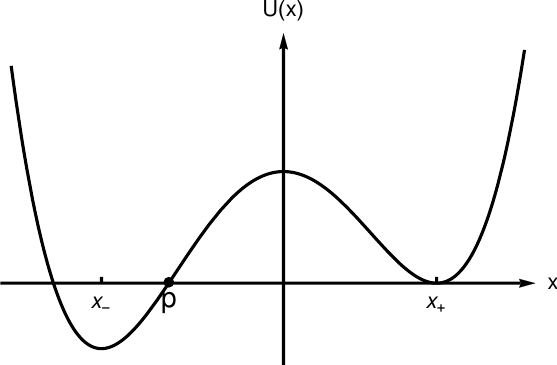
\includegraphics[scale = 0.4]{../FIGURAS/potencial}
	\caption{Potencial con un falso vacío en $x_+$ \cite{Ai:2019dqr}.}
	\label{fig:potencial}
\end{figure}

Haciendo uso de la aproximación WKB, se demuestra que $\Gamma$ es de la forma \cite{coleman1977fate}
\begin{equation} \label{eq:gamma_WKB}
	\Gamma = Ae^{-B}\qty(1 + \order{\hbar})
\end{equation}
donde 
\colorbox{yellow}{completar}
\begin{equation} \label{B_WKB}
	B = \int \dd{x} \sqrt{V} 
\end{equation}





